% Copyright 2022 Pierre S. Caboche. All rights reserved.

\renewcommand{\currentPart}{Results and Conclusion}

\newpage
\part{Results and Conclusion}

Here is a summary of what we've learned about each language, and how they performed (on the older machine, with an \Intel\ \Core~i5-8259U processor and PCI-Express 3 NVMe SSD):

\begin{itemize}
	\item \awk\ was initially developed at Bell Labs in the 1970s for the original AT\&T \Unix.	
	Its modern GNU implementation, \gawk, implements features such as regular expressions \emph{group capturing} (but not \emph{named} group capturing).
	
	GNU awk 5.1.0 processed our file in about 9 seconds (with some outliers. The very worst cases took less than 15 seconds). \\
	
	\item \perl\ was initially designed in 1987 by Larry Wall, but now the name ``Perl" refers to Perl 5, first released in 1994 after a near complete rewrite of the interpreter, and the addition of new features (including \emph{named group capturing} in regular expressions, a feature inspired by Python).
	
	Perl 5.34.1 processed our file in about 9 seconds (with some outliers. The very worst cases took less than 15 seconds). \\
	
	
	\item \python\ is a slightly more modern language, first appearing in 1991. 
	
	Python 3.10.5 processed our file in around 15 minutes, which is between 60 and 100 times longer than either \gawk\ or \perl\dots
	
	Also, due to some problems with how Python handles UTF-8, some of our data was lost. Trying to fix the issue is not an easy task, and it was actually simpler to rewrite the script in either \gawk\ or \perl\ (despite initial the learning curve).
	
	
	\item \julia\ is the most recent language, first appearing in 2012.
	 
	 \julia\ is a young but promising language, aimed to be easy to learn, very versatile, and fast. \julia's goal is to be usable for a wide array of applications, including general programming, file processing, statistics, and more\dots
	 
	 Julia 1.7.3 processed our file in about the same time as \awk\ and \perl\ (around 9 seconds). \\
	 
\end{itemize}


Later, I repeated the tests on new computer with a faster CPU (\Intel\ \Core~i5-1135G7), a faster (PCI-Express 4) NVMe SSD, and a freshly installed Linux. \\

\newpage

Below are the results:

\begin{figure}[h]
	\caption{Speed comparison of Python, AWK, and Perl}
	\medskip
	\pgfplotsset{compat=newest}
	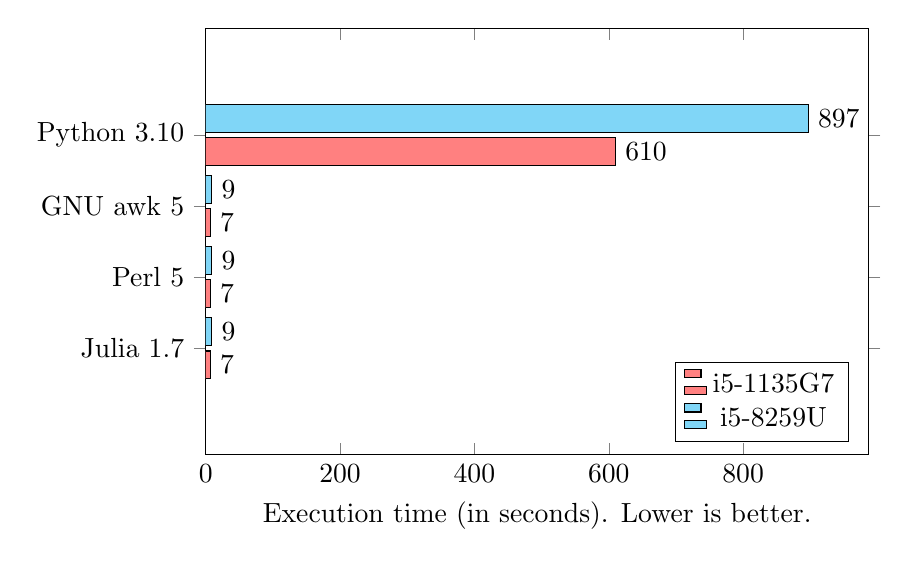
\begin{tikzpicture}
		\begin{axis}
			[ 
			xbar, 
			xmin=0, 
			width=10cm,
			height=7cm, 
			enlarge y limits=0.5, 
			xlabel={Execution time (in seconds). Lower is better.},
			%ylabel={Language},
			symbolic y coords={julia,perl,gawk,python}, 
			yticklabels={Python 3.10,GNU awk 5,Perl 5,Julia 1.7},
			ytick=data,
			nodes near coords,
			nodes near coords align={horizontal}, 
			legend pos=south east
			]
			\addplot[fill=red!50] coordinates {(610,python) (7,gawk) (7,perl) (7,julia) }; 
			\addplot[fill=cyan!50] coordinates {(897,python) (9,gawk) (9,perl) (9,julia) };
			\legend{i5-1135G7,i5-8259U};
		\end{axis} 
	\end{tikzpicture}
\end{figure}

\medskip

On the 1135G7, the scripts in \awk, \perl, and \julia\ all took between 5 and 9 seconds to execute. This difference of speed can be attributed to external factors (i.e. systems processes which run in the background and interfere with the results).

Meanwhile on the same computer, the \python\ script took 10 minutes to execute. 
Given that the \python\ script takes so long to run, a slowdown of a few seconds is barely noticeable\dots \\


\medskip

Another way to look at the results is by comparing the processing speed of each language (by dividing the input size by the total execution time). \\
 

\begin{figure}[h]
	\caption{Processing speed comparison of Python, AWK, and Perl}
	\medskip
	\pgfplotsset{compat=newest}
	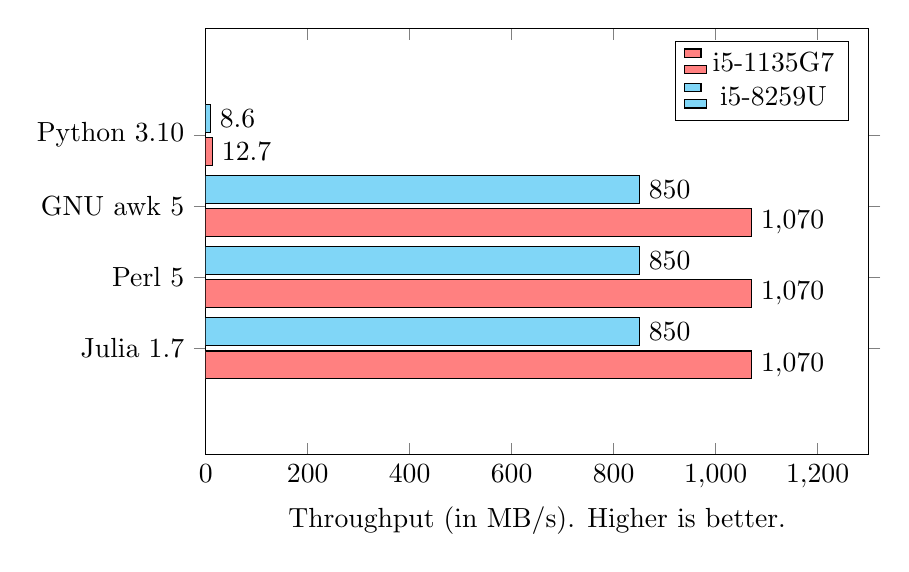
\begin{tikzpicture}
		\begin{axis}
			[ 
			xbar, 
			xmin=0, 
			width=10cm,
			height=7cm, 
			enlarge y limits=0.5, 
			xlabel={Throughput (in MB/s). Higher is better.},
			xmax=1300,
			%ylabel={Language},
			symbolic y coords={julia,perl,gawk,python}, 
			yticklabels={Python 3.10,GNU awk 5,Perl 5,Julia 1.7},
			ytick=data,
			nodes near coords,
			nodes near coords align={horizontal}, 
			legend pos=north east
			]	
			\addplot[fill=red!50] coordinates {(12.7,python) (1070,gawk) (1070,perl) (1070,julia)}; 
			\addplot[fill=cyan!50] coordinates {(8.6,python) (850,gawk) (850,perl) (850,julia)};
			\legend{i5-1135G7,i5-8259U};
		\end{axis} 
	\end{tikzpicture}
	\label{figure:throughput-comparison}
	
\end{figure}


\bigskip


In figure \ref{figure:throughput-comparison}, the difference of speed between Python and the other two languages is really striking! \\

For reference, the theoretical maximum throughput of SATA 3 is 600~MB/s. Both \awk\ and Perl process the data at a higher rate than that, and we are limited only by the CPU's single thread processing speed, not by the speed of NVMe SSD (whether it be PCI Express~3 or PCI Express~4). \\


Also worth noting:

\begin{itemize}
	
	\item We used processors of different generations: an \nth{8} generation \Intel\ \Core\ (i5-8259U), and an \nth{11} generation \Intel\ \Core\ (i5-1135G7).
	
	Between the two processors, released a little over 2 years apart (one in Q2'2018, the other in Q3'2020), we observe a 33\% difference in performance throughout the board.
	This is consistent with online benchmarks, which show a \emph{single core} performance\footnote{our scripts don't make use of multiple cores} of 37\% between the two processors \citep{userbenchmark}. \\
	
	\item Another notable difference between those two computers was the use of a much better SSD on the more recent machine.
	
	This did not impact the results (i.e. all our scripts were able to read/write as much data as they could process. Even the slower SSD did not constitute a bottleneck\footnote{in some previous test on another machine, the SSD read/write speeds were below 700 MB/s, which created a bottleneck that affected the performance of the \gawk\ and \perl\ scripts. The Python script was not impacted because it could barely process 12 MB/s.})
\end{itemize}

\bigskip

\section*{Key takeaways}

Python has a reputation for being a very slow scripting language. \\

In this paper, we showed that this reputation is highly deserved. \\

In fact, the very reason why we looked at other scripting languages (\awk, \perl, and \julia) is because \python\ was so slow that it became impractical to use in our particular use-case. 
To add insult to injury, we also ended up with some corrupted data in our output files because of the way \python\ handles UTF-8 streams. \\


Now let's review some of \python's strong points, and see if they still hold up today:

\begin{itemize}
	\item \emph{``Python is cross-platform"} \\
	
	For a long time, this was a major advantage of \python: the ability to develop a script on one system, while knowing it should be able to run on other systems.  \\
	
	
	
	\newpage
	
	This has been less relevant today, especially on Windows, thanks to Windows Subsystem for Linux which allow to run any Linux scripts on a Windows machine, with some caveats\footnote{notably, it is difficult to access a Windows service (e.g. a database) from the Linux Subsystem. In essence, WSL2 creates a Linux virtual machine which runs on a Windows host. Such virtual machine has access to the host's file system (through \cmd{/mnt}), but is seen by Windows as a separate machine, which you need to grant access to (by configuring the firewall, and allow the service to accept connection from that machine). It is not straightforward.} \\
	
	\bigskip
	
	\item \emph{``Python is very popular"} \\
	
	Being popular means that there exists a lot of resources online about \python, a great number of engineer will have \python\ on their résumé, and many job postings will also mention \python\ as a desired skill. \\
	
	What those numbers don't show is the number of companies which require \python\ because it is part of their technical stack, but are actively looking to move away from it for a reason or another.
	
	I do not have exact figures on the matter, only empirical data. That being said, it is good to ask how \python\ is used in a company, and if they are considering alternatives. \\
	
	\bigskip

	\item \emph{``Python provides a lot of libraries, especially for data analysis"}	\\
	
	In that particular domain, one scripting language to watch is \julia.
	
	Not only is \julia\ a general-purpose language very well versed in numerical analysis, but as we saw in this article, \julia\ is really fast too. \\
		
\end{itemize}

\newpage


\section*{Conclusion}


In this article, we showed some of the shortcomings of \python, and explored different alternatives. \\

Not only was \python\ frustratingly slow for processing large data files (for the purpose of cleaning up data, sorting, modifying the format, etc.), but it also corrupted some of our data (the non-valid UTF-8 characters, i.e. the binary data which was part of our file). 

We tried different alternatives, which all gave much better results for that particular use-case. \\


Here is a summary of the different languages we tried:
 
 
\begin{description}
	\item[AWK] \mbox{}  \\
	AWK is a very specialised language (designed mainly for text processing) but is very good at what it does! Its syntax is simple, even if requires a bit of getting used to it. 
	
	I personally use GNU Awk rather frequently, when dealing with large text file. I appreciate its simplicity and its speed.
	
	\item[Perl] \mbox{} \\
	\perl\ is more advanced than AWK, offering similar speed, and more features. 
	
	One of the problems of \perl\ is its syntax. \perl\ usually offers multiple ways to handle a problem, but they often relies on some specific syntax, making harder to learn (on top of the fact that different \perl\ programmers may have different coding styles)
		
	\item[Julia] \mbox{} \\
	\julia\ is probably one of the most criminally under-appreciated languages of the moment.
	
	\julia\ has a syntax that is generally easy to follow, provides access to a great number of libraries, all while delivering high execution speed.

	Of all the languages tested, \julia\ objectively possesses the most qualities:
	
	\begin{itemize}
		\item \julia's syntax is easy to learn (easier than \perl)
		\item \julia\ is very versatile (unlike \awk)
		\item \julia\ natively possesses many of the same features as \python\ (\julia\ can call \python\ libraries with PyCall.jl, or make direct calls to C and Fortran libraries)
		\item \julia\ offers great performance (on par with \awk\ and \perl)
	\end{itemize}
\end{description}

\bigskip


\awk\ still remains a very good option for file processing, because of its very simple syntax. For more complex tasks however, \julia\ should be really high on your list of languages to consider. \\

If you intent to start a \python\ project but have the possibility to choose another language, you might want to give \julia\ a try.
It is very likely that \julia\ would be able to perform the same tasks as \python, but better. \\

Hopefully this article will have given you a better understanding of the characteristics of each language, and that the examples provided would help you quickly get started and familiarise yourself with the syntax and features.

\newpage
\subsection*{Going further}

All the scripts used in this article are provided under the BSD license (please see the ``Legal" section), which is very permissive. \\

This allows you to:

\begin{enumerate}
	\item \label{get-started}
	quickly get started with processing files in \python, \awk, \perl, or \julia 

	\begin{enumerate}
		\item \label{modify-scripts}
		modify the scripts for your own data-processing needs 
	\end{enumerate}
	
	\item \label{reproduce-experiments}
	reproduce the experiments detailed in this article (i.e. separate data into different buckets) and see the results for yourself
	
	\item \label{extend-experiment}
	extend the experiment to include other languages 
\end{enumerate}

\bigskip

Regarding point \ref{get-started} (quickly getting started), our different examples are easy to follow yet cover useful programming concepts (variables, loops, conditions, I/O, files, regular expressions, etc.). 
Also, comparing the different implementations allows us to focus on what makes each language unique, and the different approaches they take in solving certain problems. \\


As far as point \ref{reproduce-experiments} is concerned (reproducing the experiments), please note that I am not at the liberty to provide you with any dataset. You will need to use your own database dump files. \\

A good dataset should contain a mix of big and small tables (in terms of number of records), wide and narrow tables (in terms of number of fields), wide and narrow data (in terms of string lengths), and potentially some binary data. \\

Finally concerning point \ref{extend-experiment}, this article started as a comparison between \python\ and \awk\ for the processing of large text files. \perl\ and \julia\ were added later on, because they are well suited for the processing of files. \\

Comparing more languages would necessitate some changes in the methodology, notably:
\begin{itemize}
	\item a standardised dataset would have to be created (see point \ref{reproduce-experiments})
	\item there is a need to distinguish between scripting languages (whose code can be easily modified) and compiled languages (which usually have the advantage of speed)
	\item one language may have more than one reference implementation. In that case, it would be necessary to compare the different alternatives
\end{itemize}
If that were to happen, this would require a separate paper, more focussed on comparing execution speed than analysing the differences in features and syntax between the different languages. \\


